\documentclass[11pt]{report}

\usepackage{preamble}

\begin{document}

\noindent \textit{Modelización} \hfill \textit{Curso 2024-2025}

\vspace{-7mm}

\begin{center}

	\rule{\textwidth}{1.6pt}\vspace*{-\baselineskip}\vspace*{2pt} % Thick horizontal rule
	\rule{\textwidth}{0.4pt} % Thin horizontal rule
	
    \vspace{3mm}

	{\LARGE \textbf{Ejercicios del Tema 4}} % Title

    \vspace{2mm}
	
	\rule[0.66\baselineskip]{\textwidth}{0.4pt}\vspace*{-\baselineskip}\vspace{3.2pt} % Thin horizontal rule
	\rule[0.66\baselineskip]{\textwidth}{1.6pt} % Thick horizontal rule

\end{center}

\begin{exercise}
    Determinar y clasificar, según su estabilidad, las soluciones de equilibrio de las siguientes ecuaciones diferenciales. Dibujar el diagrama de fases.
    \begin{enumerate}
        \item $x'=x$.
        \item $x'=-x$.
        \item $x'=x^2-1$.
        \item $x'=x^2$.
    \end{enumerate}
\end{exercise}

\begin{solution}
    Se va a omitir el dibujo de los diagramas de fases.
    \begin{enumerate}
        \item Considérese la función $f \colon \R \to \R$ dada por $f(x) = x$. Se tiene que
        \[f(x) = 0 \iff x = 0,\]
        así que el único equilibrio del sistema es $l = 0$. Como $f$ es de clase $1$ y $f'(l) = 1 > 0$, se trata de un equilibrio inestable y repulsor.
        \item Considérese la función $f \colon \R \to \R$ dada por $f(x) = -x$. Se tiene que
        \[f(x) = 0 \iff x = 0,\]
        así que el único equilibrio del sistema es $l = 0$. Como $f$ es de clase $1$ y $f'(l) = -1 < 0$, se trata de un equilibrio asintóticamente estable.
        \item Considérese la función $f \colon \R \to \R$ dada por $f(x) = x^2-1$. Se tiene que
        \[f(x) = 0 \iff x = \pm 1,\]
        así que los equilibrios del sistema son $l_1 = 1$ y $l_2 = -1$. Como $f$ es de clase $1$, $f'(l_1) = 2 > 0$ y $f'(l_2) = -2 < 0$, se tiene que $l_1$ es inestable y repulsor y $l_2$ es asintóticamente estable.
        \item Considérese la función $f \colon \R \to \R$ dada por $f(x) = x^2$. Se tiene que
        \[f(x) = 0 \iff x = 0,\]
        así que el único equilibrio del sistema es $l = 0$. Como $f$ es de clase $1$ y $f'(l) = 0$, se trata de un equilibrio no hiperbólico. Razonando geométricamente se deduce que $l$ es inestable (semiestable por la izquierda), pues $f(x) > 0$ para todo $x \neq 0$ y por tanto $x$ es estrictamente creciente en $\R$.
    \end{enumerate}
\end{solution}

\begin{exercise}
    Determinar las soluciones de equilibrio de las siguientes ecuaciones y su estabilidad. Dibujar el diagrama de fases.
    \begin{enumerate}
        \item $x' = ax+bx^2, \ a > 0, \ b > 0$.
        \item $x' = x(x-1)(x-2)$.
        \item $x' = e^x-1$.
        \item $x' = e^{-x}-1$.
    \end{enumerate}
\end{exercise}

\begin{solution}
    Se va a omitir el dibujo de los diagramas de fases.
    \begin{enumerate}
        \item Considérese la función $f \colon \R \to \R$ dada por $f(x) = ax+bx^2$. Se tiene que
        \[f(x) = 0 \iff x = 0 \textup{ ó } x = -\frac{a}{b},\]
        así que los equilibrios del sistema son $l_1 = 0$ y $l_2 = -\frac{a}{b}$. Se tiene que $f$ es de clase $1$, $f'(l_1) = a>0 $ y $f'(l_2) = a-2b\frac{a}{b} = -a < 0$. Por tanto, $l_1$ es inestable y repulsor y $l_2$ es asintóticamente estable.
        \item Considérese la función $f \colon \R \to \R$ dada por $f(x) = x(x-1)(x-2) = x^3-3x^2+2x$. Se tiene que
        \[f(x) = 0 \iff x = 0, \ x = 1 \textup{ ó } x = 2,\]
        así que los equilibrios del sistema son $l_1 = 0$, $l_2 = 1$ y $l_2 = 2$. Se tiene que $f$ es de clase $1$ y $f'(x) = 3x^2-6x+2$. Por tanto, $f'(l_1) = 2 > 0$, $f'(l_2) = -1 < 0$ y $f'(l_3) = 2 > 0$, luego $l_1$ y $l_3$ son inestables y repulsores y $l_2$ es asintóticamente estable.
        \item Considérese la función $f \colon \R \to \R$ dada por $f(x) = e^x-1$. Se tiene que
        \[f(x) = 0 \iff x = 0,\]
        así que el único equilibrio del sistema es $l = 0$. Se tiene que $f$ es de clase $1$ y $f'(l) = 1 > 0$, así que $l$ es inestable y repulsor.
        \item Considérese la función $f \colon \R \to \R$ dada por $f(x) = e^{-x}-1$. Se tiene que
        \[f(x) = 0 \iff x = 0,\]
        así que el único equilibrio del sistema es $l = 0$. Se tiene que $f$ es de clase $1$ y $f'(l) = -1 < 0$, así que $l$ es asintóticamente estable.
    \end{enumerate}
\end{solution}

\begin{exercise}
    Determinar las soluciones de equilibrio de las siguientes ecuaciones y su estabilidad. Dibujar el diagrama de fases.
    \begin{enumerate}
        \item $x' = \sen(x)$.
        \item $x' = k(1-x)^2, \ k > 0$.
        \item $x' = -k(x-1)^2, \ k > 0$.
        \item $x' = x^2(x^2-1)$.
        \item $x' = x(1-x^2)$.
    \end{enumerate}
\end{exercise}

\begin{solution}
    Se va a omitir el dibujo de los diagramas de fases.
    \begin{enumerate}
        \item Considérese la función $f \colon \R \to \R$ dada por $f(x) = \sen(x)$. Se tiene que
        \[f(x) = 0 \iff x = k\pi, \ k \in \Z,\]
        así que los equilibrios del sistema son $l_k = k\pi$, $k \in \N$. Se tiene que $f$ es de clase $1$ y $f'(l_k) = \cos(k\pi) = (-1)^k$, así que $l_k$ es asintóticamente estable si $k$ es impar, e inestable y repulsor si $k$ es par.
        \item Considérese la función $f \colon \R \to \R$ dada por $f(x) = k(1-x)^2$. Se tiene que
        \[f(x) = 0 \iff x = 1,\]
        así que el único equilibrio del sistema es $l = 1$. Se tiene que $f$ es de clase $1$ y $f'(l) = 0$, así que $l$ es un equilibrio no hiperbólico. Razonando geométricamente se deduce que $l$ es inestable (semiestable por la izquierda), pues $f(x) > 0$ para todo $x \neq 1$.
        \item Considérese la función $f \colon \R \to \R$ dada por $f(x) = -k(x-1)^2$. Se tiene que
        \[f(x) = 0 \iff x = 1,\]
        así que el único equilibrio del sistema es $l = 1$. Se tiene que $f$ es de clase $1$ y $f'(l) = 0$, así que $l$ es un equilibrio no hiperbólico. Razonando geométricamente se deduce que $l$ es inestable (semiestable por la derecha), pues $f(x) < 0$ para todo $x \neq 1$.
        \item Considérese la función $f \colon \R \to \R$ dada por $f(x) = x^2(x^2-1)$. Se tiene que
        \[f(x) = 0 \iff x = 0, \ x = 1 \textup{ ó } x = -1,\]
        así que los equilibrios del sistema son $l_1 = 0$, $l_2 = 1$ y $l_3 = -1$. Se tiene que $f$ es de clase $1$ y $f'(x) = 4x^3-2x$. Por tanto, $f'(l_1) = 0$, $f'(l_2) = 2 > 0$ y $f'(l_3) = -2 < 0$, así que $l_1$ es un equilibrio no hiperbólico, $l_2$ es inestable y repulsor y $l_3$ es asintóticamente estable. Razonando geométricamente se deduce que $l_1$ es inestable (semiestable por la derecha), pues existe $\varepsilon > 0$ tal que $f(x) < 0$ para todo $x \in (-\varepsilon,\varepsilon) \setminus\{0\}$. 
        \item Considérese la función $f \colon \R \to \R$ dada por $f(x) = x(1-x^2)$. Se tiene que
        \[f(x) = 0 \iff x = 0, \ x = 1 \textup{ ó } x = -1,\]
        así que los equilibrios del sistema son $l_1 = 0$, $l_2 = 1$ y $l_3 = -1$. Se tiene que $f$ es de clase $1$ y $f'(x) = 1-3x^2$. Por tanto, $f'(l_1) = 1 > 0$, $f'(l_2) =-2 < 0$ y $f'(l_3) = -2 < 0$, así que $l_1$ es inestable y repulsor y $l_2$ y $l_3$ son asintóticamente estables. 
    \end{enumerate}
\end{solution}

\begin{exercise}
    Determinar las soluciones de equilibrio de las siguientes ecuaciones y su estabilidad. Dibujar el diagrama de fases.
    \begin{enumerate}
        \item $x' = ax-b\sqrt{x}, \ a > 0, \ b > 0$.
        \item $x' = x^2(1-x)^2$.
    \end{enumerate}
\end{exercise}

\begin{solution}
    Se va a omitir el dibujo de los diagramas de fases.
    \begin{enumerate}
        \item Considérese la función $f \colon [0,\infty) \to \R$ dada por $f(x) = ax-b\sqrt{x}$. Se tiene que
        \[f(x) = 0 \iff x = 0 \textup{ ó } x=\frac{b^2}{a^2}, \]
        así que los equilibrios del sistema son $l_1 = 0$ y $l_2 = \frac{b^2}{a^2}$. Se tiene que $f$ es de clase $1$ en $(0,\infty)$ y $f'(x) = a-\frac{b}{2\sqrt{x}}$, luego $f'(l_2) = \frac{a}{2} > 0$ y por tanto $l_2$ es inestable y repulsor. Razonando geométricamente se deduce que $l_1$ es inestable (semiestable por la derecha), pues $f(x) < 0$ si y solo si $x < \frac{b^2}{a^2}$ y por tanto existe $\varepsilon > 0$ tal que $f(x) < 0$ para todo $x \in (0,\varepsilon)$.
        \item Considérese la función $f \colon \R \to \R$ dada por $f(x) = x^2(1-x)^2$. Se tiene que
        \[f(x) = 0 \iff x = 0 \textup{ ó } x=1, \]
        así que los equilibrios del sistema son $l_1 = 0$ y $l_2 = 1$. Se tiene que $f$ es de clase $1$ y $f'(x) = 2x(1-x)^2-2x^2(1-x)$, luego $f'(l_1) = f'(l_2) = 0$ y por tanto $l_1$ y $l_2$ son equilibrios no hiperbólicos. Razonando geométricamente se deduce que $l_1$ y $l_2$ son inestables (semiestables por la izquierda), pues $f(x) > 0$ para todo $x \in \R\setminus\{0,1\}$.
    \end{enumerate}
\end{solution}

\begin{exercise}
    Buscar una ecuación diferencial $x'=f(x)$ cuyo diagrama de fases conste de una única órbita que ocupe toda la recta real.
\end{exercise}

\begin{solution}
    Se trata de tomar $f$ de manera que para cada $x_0\in\R$, el problema de Cauchy
    \[(P) \ \begin{cases}
        x'(t)=f(x(t)), \qquad t \in\R, \\
        x(0) = x_0,
    \end{cases}\]
    tenga solución única y esta solución verifique $x(\R) = \R$. Esto último equivale a que $x$ sea inyectiva. Como $x'=f$, puede tomarse $f > 0$ y se tendrá que $x$ es estrictamente creciente. También se buscará que $f$ sea continua y de Lipschitz para que el problema tenga solución única.

    Sea $f \colon \R \to \R$ la función dada por $f(x) =|x+1|$. Para $x,y\in\R$ cualesquiera, se verifica $|f(x)-f(y)| = ||x+1|-|y+1||\leq |x+1-y-1| = |x-y|$. Por tanto, $f$ es de Lipschitz, y como también es continua, el problema $(P)$ tiene solución única para todo $x_0\in\R$. Además, $f(x) >0$ para todo $x \in\R$, luego dicha solución es inyectiva, pues es estrictamente creciente.

    Se concluye que la única órbita del sistema dinámico continuo dado por la función $f$ es la recta real.
\end{solution}

\begin{exercise}
    Buscar una ecuación diferencial $x'=f(x)$ cuyo diagrama de fases sea el de la siguiente figura:
    \begin{figure}[H]
        \centering
        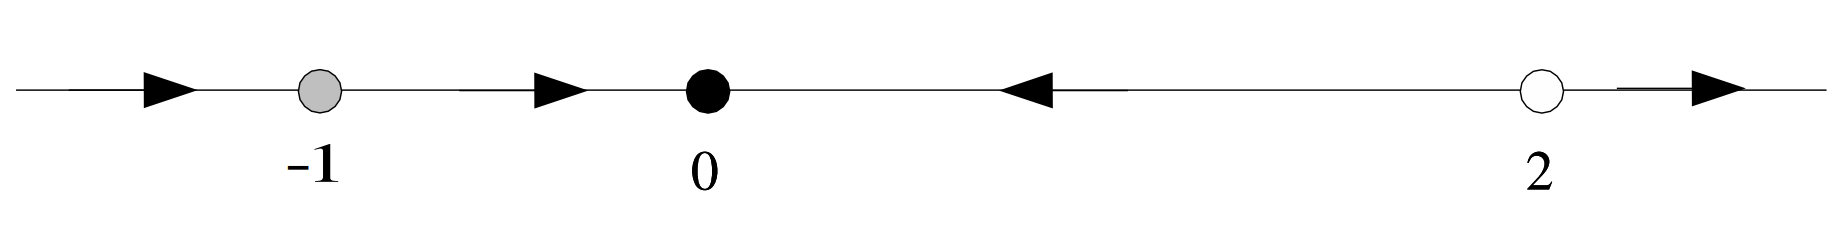
\includegraphics[scale = 0.2]{img/1.png}
    \end{figure}
\end{exercise}

\begin{solution}
    Lo más natural es considerar funciones de la forma $f(x) = x^{i}(x+1)^{j}(x-2)^k$, con $i,j,k\in\N$. Se trata de buscar una función cuya gráfica se asemeje a la siguiente:
    \begin{figure}[H]
        \centering
        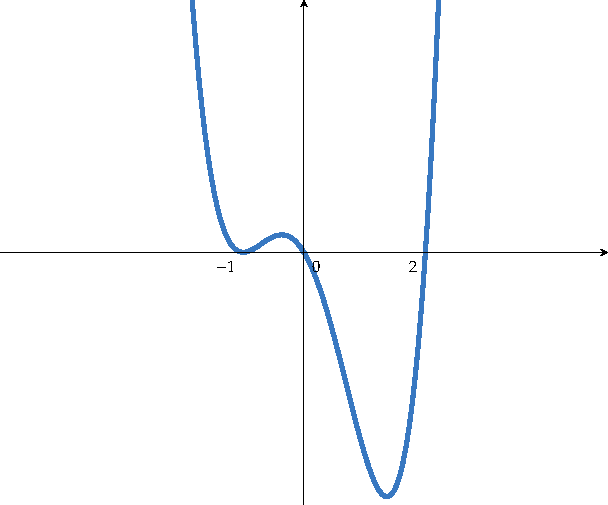
\includegraphics[scale = 0.7]{plot1/main.pdf}
    \end{figure}
    Basta tomar $f(x) = x(x+1)^2(x-2)$.
\end{solution}

\begin{exercise}
    Encontrar una ecuación diferencial $x'=f(x)$ cuyas soluciones sean consistentes con la siguiente figura:
    \begin{figure}[H]
        \centering
        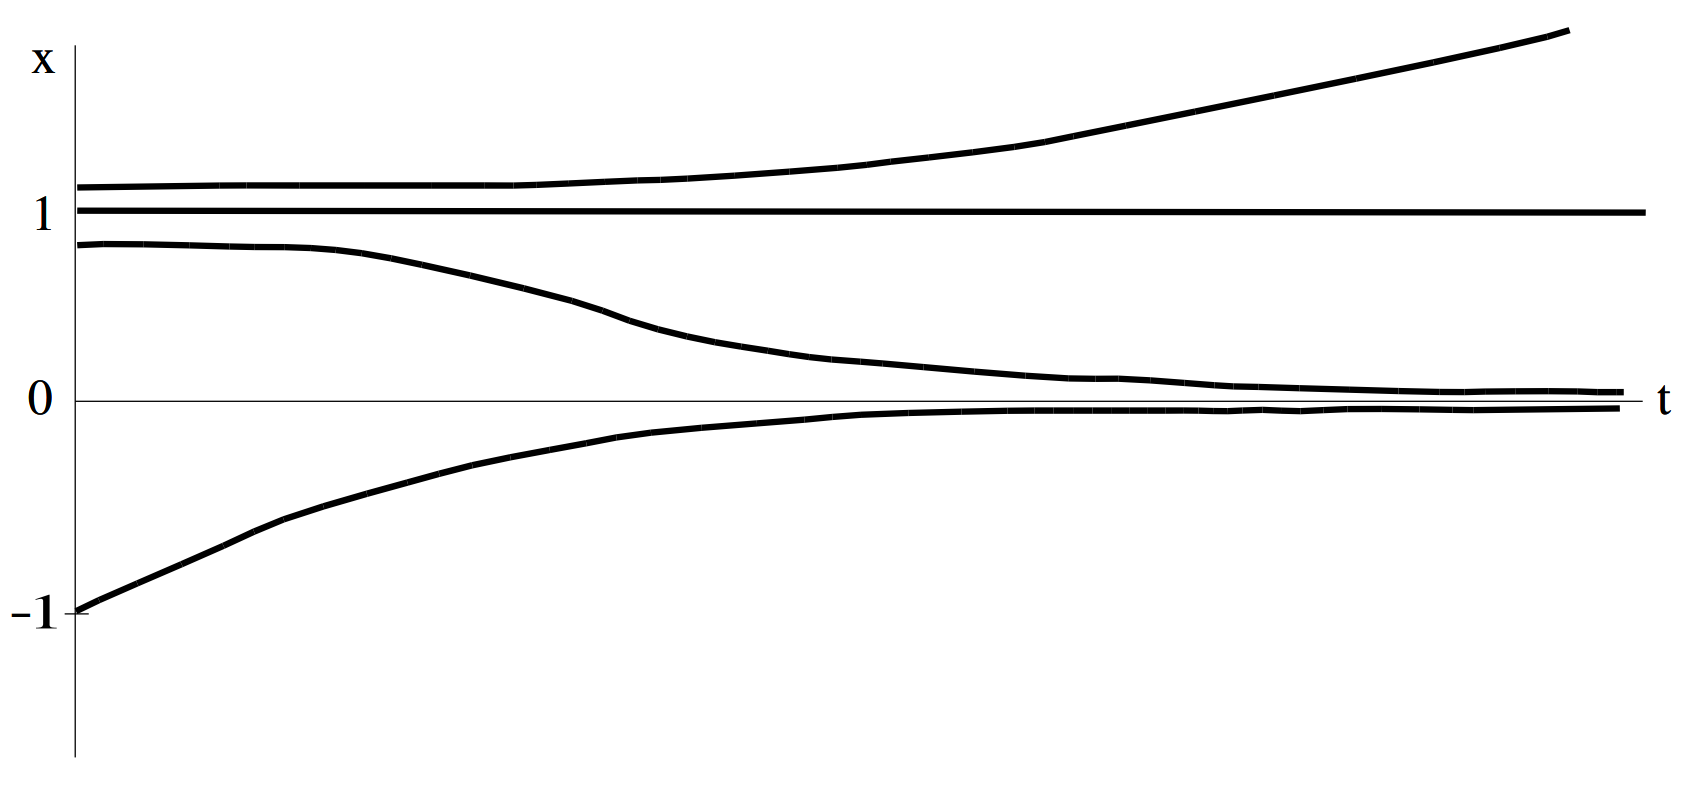
\includegraphics[scale = 0.2]{img/2.png}
    \end{figure}
\end{exercise}

\begin{solution}
    La función $f$ debe verificar las siguientes propiedades:
    \begin{itemize}
        \item $f(0) = f(1) = 0$, para que las soluciones constantes sean $x \equiv 0$ y $x \equiv 1$.
        \item $f(x) > 0$ para todo $x \in(1,\infty)$, para que las soluciones cuya gráfica esté contenida en $[0,\infty)\times(1,\infty)$ sean estrictamente crecientes.
        \item $f(x) < 0$ para todo $x \in (0,1)$, para que las soluciones cuya gráfica esté  contenida en $[0,\infty)\times(0,1)$ sean estrictamente decrecientes.
        \item $f(x) > 0$ para todo $x \in [-1,0)$, para que las soluciones cuya gráfica esté contenida en $[0,\infty)\times[-1,0)$ sean estrictamente crecientes.
    \end{itemize}
    Se trata de buscar una función cuya gráfica se asemeje a la siguiente:
    \begin{figure}[H]
        \centering
        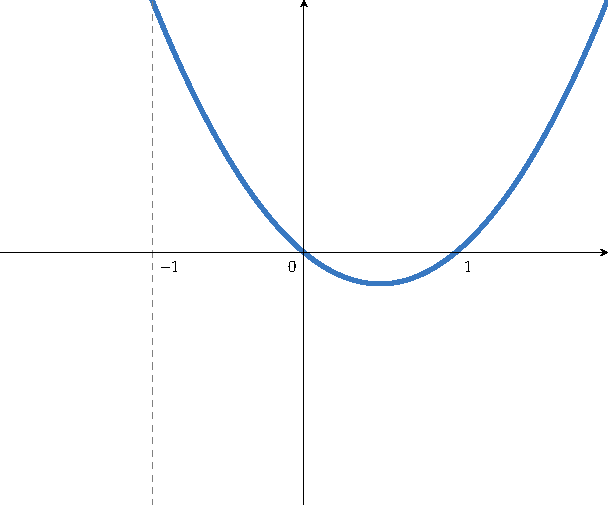
\includegraphics[scale = 0.7]{plot2/main.pdf}
    \end{figure}
    Basta escoger $f(x) = x(x-1)$.
\end{solution}

\begin{exercise}
    En los siguientes casos, encontrar una ecuación diferencial $x'=f(x)$ con las propiedades que se especifican (en caso de que no haya ejemplos, explicar por qué):
    \begin{enumerate}
        \item Todo número real es un punto de equilibrio.
        \item Todo entero es un punto de equilibrio, y no hay ninguno más.
        \item Hay exactamente tres puntos de equilibrio, todos ellos estables.
        \item No hay puntos de equilibrio.
        \item Hay exactamente 100 puntos de equilibrio.
    \end{enumerate}
\end{exercise}

\begin{solution}
    \hfill
    \begin{enumerate}
        \item Basta tomar $f \equiv 0$. Todo número real es un cero de $f$, y por tanto es un punto de equilibrio.
        \item Basta tomar $f(x) = \sen(\pi x)$, $x \in \R$. Se tiene que
        \[f(x) = 0 \iff \pi x = k\pi, \ k \in \Z \iff x = k, \ k \in \Z \iff x \in \Z,\]
        así que los únicos puntos de equilibrio son los números enteros.
        \item Es imposible que haya tres puntos de equilibrio estables, pues no pueden haber dos equilibros estables consecutivos. Por reducción al absurdo, sean $l_1,l_2 \in \R$ dos equilibrios consecutivos estables de $f$ con $l_1<l_2$. Entonces existen $\varepsilon_1,\varepsilon_2>0$ tales que $f(x) > 0$ para todo $x \in (l_1-\varepsilon_1,l_1) \cup (l_2-\varepsilon_2,l_2)$ y $f(x) < 0$ para todo $x \in (l_1,l_1+\varepsilon_1) \cup (l_2,l_2+\varepsilon_2)$. Tomando $\varepsilon_1$ y $\varepsilon_2$ más pequeños si fuera necesario, puede suponerse que $l_1+\varepsilon_1<l_2-\varepsilon_2$.  Como $f(x) > 0$ para todo $x \in (l_1,l_1+\varepsilon_1)$ y $f(x) < 0$ para todo $x \in (l_2-\varepsilon_2,l_2)$, por el teorema de Bolzano, existe $l \in [l_1+\varepsilon_1,l_2+\varepsilon_2]$ tal que $f(l) = 0$. Esto contradice que $l_1$ y $l_2$ sean dos equilibrios consecutivos.
        \item Basta tomar $f(x) = x^2+1$, que satisface $f(x)>0$ para todo $x \in \R$ y por tanto no proporciona puntos de equilibrio.
        \item Basta tomar $f(x) = \prod_{i=1}^{100}(x-i)$, que tiene exactamente $100$ ceros.
    \end{enumerate}
\end{solution}

\begin{exercise}
    Dado un número real $\mu$, se considera la función
    \[f_\mu(x) = x^2-\mu x.\]
    Dibujar el diagrama de bifurcación de la familia de ecuaciones diferenciales ordinarias
    \[x'=f_\mu(x).\]
\end{exercise}

\begin{solution}
    Se tiene que
    \[f_\mu(x) = 0 \iff x = 0 \textup{ ó } x = \mu.\]
    Por tanto, el conjunto de los equilibrios de la familia de ecuaciones dada es
    \[\{(\mu,0)  \in\R^2\colon \mu \in \R\} \cup \{(x,x) \in\R^2\colon x \neq 0\}\]
    Por otra parte, $f'(x) = 2x-\mu$, luego $f'(0) = -\mu$ y $f'(\mu) = \mu$.
    \begin{itemize}
        \item Si $\mu < 0$, los equilibrios del sistema son $l_1 = 0$ y $l_2 = \mu$. Se tiene que $l_1$ es inestable y repulsor, y $l_2$ es asintóticamente estable.
        \item Si $\mu > 0$, los equilibrios del sistema son $l_1 = 0$ y $l_2 = \mu$. Se tiene que $l_1$ es asintóticamente estable, y $l_2$ es inestable y repulsor.
        \item Si $\mu = 0$, el único equilibrio del sistema es $l = 0$, que no es hiperbólico.
    \end{itemize}
    \begin{figure}[H]
        \centering
        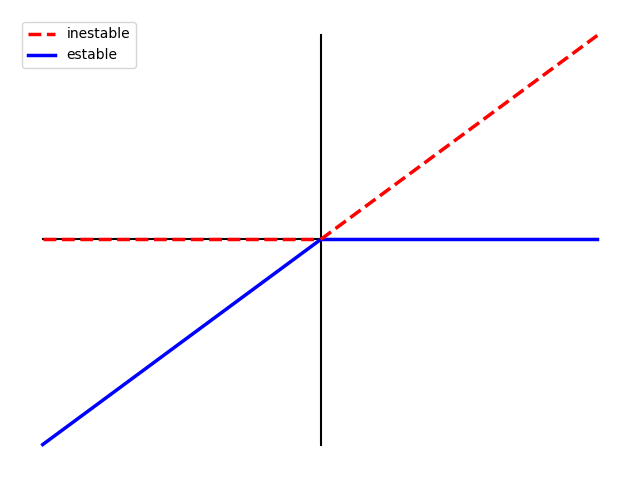
\includegraphics[scale=0.5]{img/3.png}
    \end{figure}
\end{solution}

\begin{exercise}
    Se considera la ecuación diferencial
    \[\frac{dx}{dt} = (R-R_c)x-a x^3.\]
    En este problema consideraremos $R_c$ y $a$ como dos constantes positivas fijas, mientras que $R$ es un parámetro que puede tomar distintos valores; es decir, consideramos una familia uniparamétrica de ecuaciones diferenciales, con un parámetro $R$.
    \begin{enumerate}
        \item Si $R<R_c$, probar que hay una única solución de equilibrio, que es estable.
        \item Si $R>R_c$, probar que hay tres soluciones de equilibrio. Estudiar su estabilidad.
        \item Dibujar el diagrama de bifurcación.
    \end{enumerate}
\end{exercise}

\begin{solution}
    Para cada $R\in\R$, sea $f_R(x) = (R-R_c)x-a x^3 = -x(ax^2-R+R_c)$.
    \begin{enumerate}
        \item Si $R<R_c$, entonces $ax^3-R+R_c >0$ para todo $x\in\R$, así que $f_R(x) = 0$ si y solo si $x = 0$. En consecuencia, solo hay una solución de equilibrio, que es $l = 0$. Como $f_R'(0) = R-R_c <0$, dicho equilibrio es asintóticamente estable.
        \item Si $R > R_c$, entonces
        \[f_R(x) = 0 \iff x = 0, x = \sqrt{\frac{R-R_c}{a}} \textup{ ó } x = -\sqrt{\frac{R-R_c}{a}},\]
        así que hay tres soluciones de equilibrio: $l_1 = 0$, $l_2 = \sqrt{\frac{R-R_c}{a}} $ y $l_3 = -\sqrt{\frac{R-R_c}{a}}$. Como $f_R'(x) = R-R_c-3ax^2$, entonces
        \begin{itemize}
            \item $f_R'(l_1) = R-R_c > 0$, así que $l_1$ es inestable y repulsor;
            \item $f_R'(l_2) = R-R_c-3(R-R_c) = -2(R-R_c) < 0$, así que $l_2$ es asintóticamente estable.
            \item $f_R'(l_3) = R-R_c-3(R-R_c) = -2(R-R_c) < 0$, así que $l_3$ es asintóticamente estable.
        \end{itemize}
        \item Para representar el diagrama de bifurcación, se va a tomar $R = 1$  y $a = 1$.
    \begin{figure}[H]
        \centering
        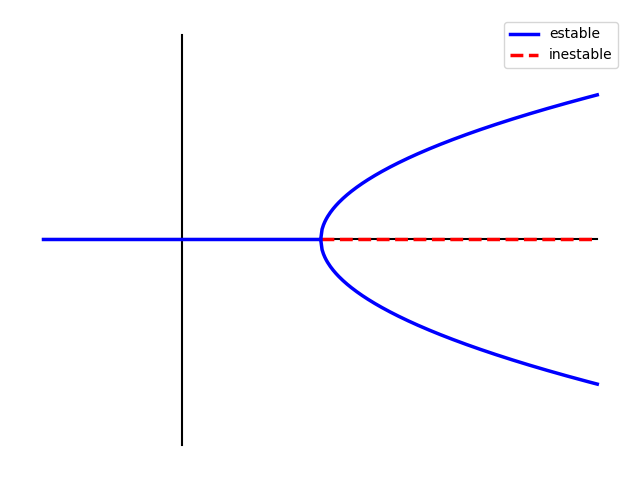
\includegraphics[scale=0.5]{img/4.png}
    \end{figure}
    \end{enumerate}
\end{solution}

\begin{exercise}
    Determinar el comportamiento cualitativo de los sistemas que se indican a continuación. En cada caso, dibujar el correspondiente diagrama de bifurcación.
    \begin{enumerate}
        \item $x'=1+\mu x + x^2$.
        \item $x' = \mu - \cosh(x)$.
    \end{enumerate}
\end{exercise}

\begin{solution}
    Solo se va a resolver el apartado (a). Sea $f_\mu(x) = 1+\mu x + x^2$. Se tiene que
    \[f_\mu(x) = 0 \iff x = \frac{-\mu\pm \sqrt{\mu^2-4}}{2}.\]
    Además, $f_\mu'(x) = \mu+2x$. Se distinguen los siguientes casos:
    \begin{itemize}
        \item Si $\mu^2-4 < 0$, es decir, si $\mu \in (-2,2)$, entonces el sistema no tiene equilibrios.
        \item Si $\mu^2-4 > 0$, es decir, si $\mu \in (-\infty,-2)\cup(2,\infty)$, entonces el sistema tiene dos equilibrios, que son \[l_1 = \frac{\sqrt{\mu^2-4}-\mu}{2} \qquad \textup{y} \qquad l_2 = -\frac{\sqrt{\mu^2-4}+\mu}{2}.\] Como $f_\mu'(l_1) = \mu +\sqrt{\mu^2-4}-\mu =\sqrt{\mu^2-4} > 0$ y $f_\mu'(l_2) = \mu -\sqrt{\mu^2-4}-\mu =  -\sqrt{\mu^2-4} < 0$, se tiene que $l_1$ es inestable y repulsor y $l_2$ es asintóticamente estable.
        \item Si $\mu^2-4 = 0$, es decir, si $\mu = -2$ o $\mu = 2$, entonces el sistema tiene un único equilibrio, que es $l = -\frac{\mu}{2}$. Como $f_\mu'(l) = \mu -\frac{2\mu}{2} = 0$, este equilibrio es no hiperbólico. Como $f(x) > 0$ para todo $x \neq l$, entonces $l$ es semiestable por la izquierda.
    \end{itemize}
    \begin{figure}[H]
        \centering
        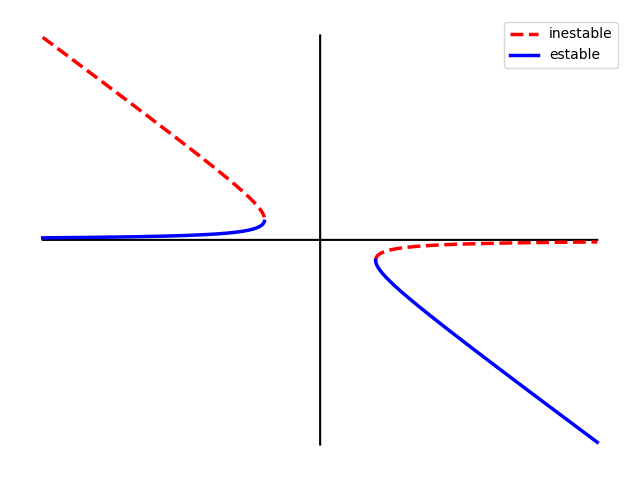
\includegraphics[scale=0.5]{img/5.png}
    \end{figure}
\end{solution}

\begin{exercise}
    Ídem para
    \begin{enumerate}
        \item $x' = \mu + x - \log(1+x)$.
        \item $x' = \mu + \frac{x}{2} - \frac{x}{1+x}$.
    \end{enumerate}
\end{exercise}

\begin{solution}
    Solo se va a resolver el apartado (b). Sea $f(\mu,x) = \mu+\frac{x}{2}-\frac{x}{1+x}$. Se tiene que
    \begin{align*}
        f(\mu,x) = 0 \iff \mu = \frac{x}{1+x}-\frac{x}{2}.
    \end{align*}
    Por tanto, el conjunto de los equilibrios del sistema es
    \[\bigl\{\bigl(\frac{x}{1+x}-\frac{x}{2},x\bigr) \in\R^2 \colon x \neq -1\bigr\}.\]
    Además, $\frac{\partial f}{\partial x}(\mu,x) = \frac{1}{2}-\frac{1+x-x}{(1+x)^2} = \frac{1}{2}-\frac{1}{(1+x)^2}$. Se tiene que
    \begin{align*}
        \frac{\partial f}{\partial x}\bigl(\frac{x}{1+x}-\frac{x}{2},x\bigr) &> 0 \iff \frac{1}{2}-\frac{1}{(1+x)^2} > 0 \iff \frac{1}{(1+x)^2} < \frac{1}{2} \iff (1+x)^2 > 2 \\
        &\iff x^2+2x-1 > 0 \iff (x+1-\sqrt{2})(x+1+\sqrt{2}) > 0 \\
        &\iff x \in (-\infty,-1-\sqrt{2}) \cup(-1+\sqrt{2},\infty).
    \end{align*}
    Asimismo,
    \begin{align*}
        \frac{\partial f}{\partial x}\bigl(\frac{x}{1+x}-\frac{x}{2},x\bigr) &< 0 \iff x \in (-1-\sqrt{2},-1+\sqrt{2}) \setminus\{-1\}.
    \end{align*}
    En consecuencia, el conjunto de los equilibrios asintóticamente estables e hiperbólicos es
    \[\bigl\{\bigl(\frac{x}{1+x}-\frac{x}{2},x\bigr) \in\R^2 \colon x\in (-1-\sqrt{2},-1+\sqrt{2}) \setminus\{-1\} \bigr\},\]
    mientras que el conjunto de los equilibrios inestables, repulsores e hiperbólicos es
    \[\bigl\{\bigl(\frac{x}{1+x}-\frac{x}{2},x\bigr) \in\R^2 \colon x \in (-\infty,-1-\sqrt{2}) \cup(-1+\sqrt{2},\infty) \bigr\}.\]
    Los equilibrios $(\frac{-1-\sqrt{2}}{-\sqrt{2}}-\frac{-1-\sqrt{2}}{2}, -1-\sqrt{2})$ y $(\frac{-1+\sqrt{2}}{\sqrt{2}}-\frac{-1+\sqrt{2}}{2}, -1+\sqrt{2})$ son no hiperbólicos.
    \begin{figure}[H]
        \centering
        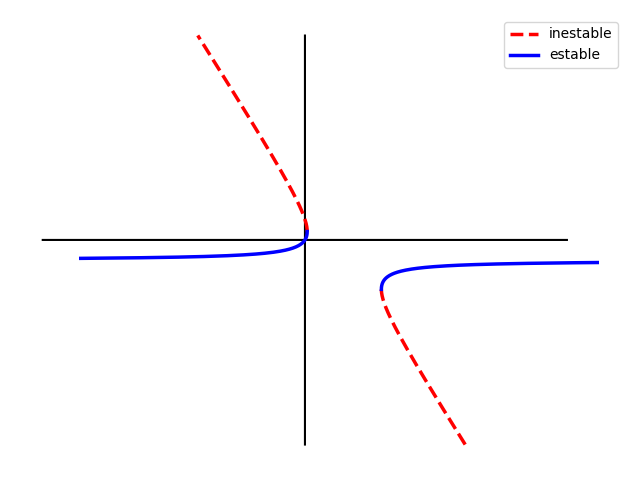
\includegraphics[scale=0.5]{img/6.png}
    \end{figure}
\end{solution}

\begin{exercise}
    Ídem para
    \begin{enumerate}
        \item $x' = \mu x + x^2$.
        \item $x' = \mu x -\log(1+x)$.
    \end{enumerate}
\end{exercise}

\begin{solution}
    Solo se va a resolver el apartado (a). Sea $f(\mu,x) = \mu x + x^2$. Se tiene que
    \begin{align*}
        f(\mu,x) = 0 \iff x = 0 \textup{ ó } x = -\mu.
    \end{align*}
    Por tanto, el conjunto de los equilibrios del sistema es
    \[\{(\mu,0) \in\R^2 \colon \mu \in \R\} \cup \{(\mu,-\mu) \in\R^2 \colon \mu \neq 0\}.\]
    Además, $\frac{\partial f}{\partial x}(\mu,x) = \mu+2x$. Se tiene que \[\frac{\partial f}{\partial x}(\mu,0) = \mu, \qquad \qquad \frac{\partial f}{\partial x}(\mu,-\mu) = \mu-2\mu = -\mu,\] así que el conjunto de los equilibrios asintóticamente estables e hiperbólicos es
    \[\{(\mu,0) \in\R^2 \colon \mu < 0\} \cup \{(\mu,-\mu) \in\R^2 \colon \mu > 0\},\]
    mientras que el conjunto de los equilibrios inestables, repulsores e hiperbólicos es
    \[\{(\mu,0) \in\R^2 \colon \mu > 0 \} \cup \{(\mu,-\mu) \in\R^2 \colon \mu < 0\}.\]
    El equilibrio $(0,0)$ no es hiperbólico. De la gráfica de $f(0,x) = x^2$ se deduce que $(0,0)$ es semiestable por la izquierda.
    \begin{figure}[H]
        \centering
        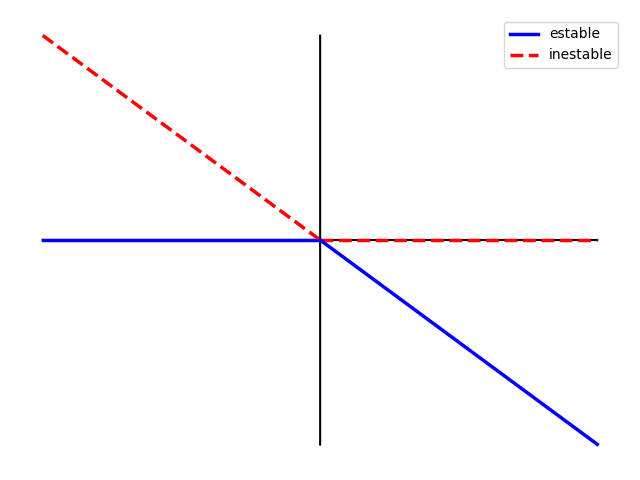
\includegraphics[scale=0.5]{img/7.png}
    \end{figure}
\end{solution}

\begin{exercise}
    Ídem para
    \begin{enumerate}
        \item $x' = x-\mu x(1-x)$.
        \item $x' = x(\mu-e^x)$.
    \end{enumerate}
\end{exercise}

\begin{solution}
    Solo se va a resolver el apartado (b). Sea $f(\mu,x) = x(\mu-e^x)$. Se tiene que
    \begin{align*}
        f(\mu,x) = 0 \iff x = 0 \textup{ ó } x = \log(\mu).
    \end{align*}
    Por tanto, el conjunto de los equilibrios del sistema es
    \[\{(\mu,0) \in\R^2 \colon \mu \in \R\} \cup \{(\mu,\log(\mu)) \in\R^2 \colon \mu > 0\}.\]
    Además, $\frac{\partial f}{\partial x}(\mu,x) = \mu-e^x-xe^x$. Se tiene que $\frac{\partial f}{\partial x}(\mu,0) = \mu-1$ para todo $\mu\in\R$, mientras que $\frac{\partial f}{\partial x}(\mu,\log(\mu)) = \mu-\mu-\mu\log(\mu) = -\mu\log(\mu)$ para todo $\mu > 0$. Por tanto, el conjunto de los equilibrios asintóticamente estables e hiperbólicos es
    \[\{(\mu,0) \in\R^2 \colon \mu < 1\} \cup \{(\mu,\log(\mu)) \in\R^2 \colon \mu > 1\},\]
    mientras que el conjunto de los equilibrios inestables, repulsores e hiperbólicos es
    \[\{(\mu,0) \in\R^2 \colon \mu > 1\} \cup \{(\mu,\log(\mu)) \in\R^2 \colon 0 < \mu < 1\},\]
    El equilibrio $(1,0)$ no es hiperbólico. Observando la gráfica de $f(1,x) = x(1-e^x)$ se deduce que $(1,0)$ es semiestable por la derecha.
    \begin{figure}[H]
        \centering
        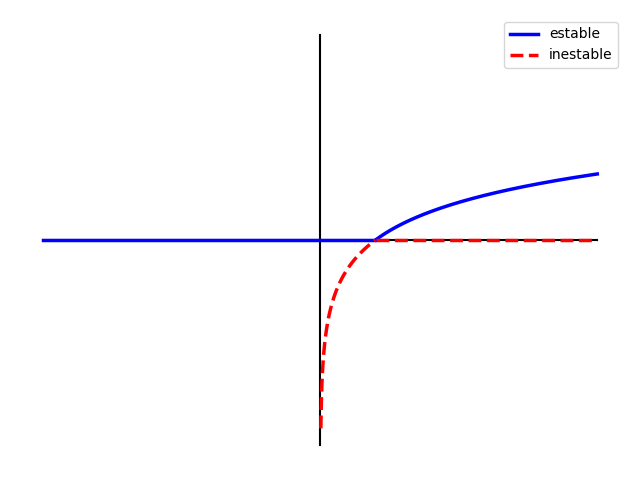
\includegraphics[scale=0.5]{img/8.png}
    \end{figure}
\end{solution}

\begin{exercise}
    Ídem para
    \begin{enumerate}
        \item $x' = \mu x +4x^3$.
        \item $x' = \mu x -\senh(x)$.
    \end{enumerate}
\end{exercise}

\begin{solution}
    Solo se va a resolver el apartado (a). Sea $f(\mu,x) = \mu x + 4x^3$. Se tiene que
    \begin{align*}
        f(\mu,x) = 0 \iff x = 0, x = \frac{\sqrt{-\mu}}{2} \textup{ ó } x = -\frac{\sqrt{-\mu}}{2}.
    \end{align*}
    Por tanto, el conjunto de los equilibrios del sistema es
    \[\{(\mu,0) \in\R^2 \colon \mu \in \R\} \cup \bigl\{\bigl(\mu, \frac{\sqrt{-\mu}}{2}\bigr) \in\R^2 \colon \mu < 0\bigr\} \cup \bigl\{\bigl(\mu, -\frac{\sqrt{-\mu}}{2}\bigr) \in\R^2 \colon \mu < 0\bigr\}.\]
    Además, $\frac{\partial f}{\partial x}(\mu,x) = \mu+12x^2$. Se tiene que $\frac{\partial f}{\partial x}(\mu,0) = \mu$ para todo $\mu\in\R$, mientras que \[\frac{\partial f}{\partial x}\bigl(\mu,\frac{\sqrt{-\mu}}{2}\bigr) = \mu-\frac{12\mu}{2} = -5\mu \qquad \textup{y} \qquad \frac{\partial f}{\partial x}\bigl(\mu,-\frac{\sqrt{-\mu}}{2}\bigr) = \mu-\frac{12\mu}{2} = -5\mu\] para todo $\mu < 0$. Por tanto, el conjunto de los equilibrios asintóticamente estables e hiperbólicos es
    \[\{(\mu,0) \in\R^2 \colon \mu < 0\},\]
    mientras que el conjunto de los equilibrios inestables, repulsores e hiperbólicos es
    \[\{(\mu,0) \in\R^2 \colon \mu > 0\} \cup \bigl\{\bigl(\mu, \frac{\sqrt{-\mu}}{2}\bigr) \in\R^2 \colon \mu < 0\bigr\} \cup \bigl\{\bigl(\mu, -\frac{\sqrt{-\mu}}{2}\bigr) \in\R^2 \colon \mu < 0\bigr\}.\]
    El equilibrio $(0,0)$ no es hiperbólico. Observando la gráfica de $f(0,x) = 4x^3$ se deduce que $(0,0)$ es inestable y repulsor.
    \begin{figure}[H]
        \centering
        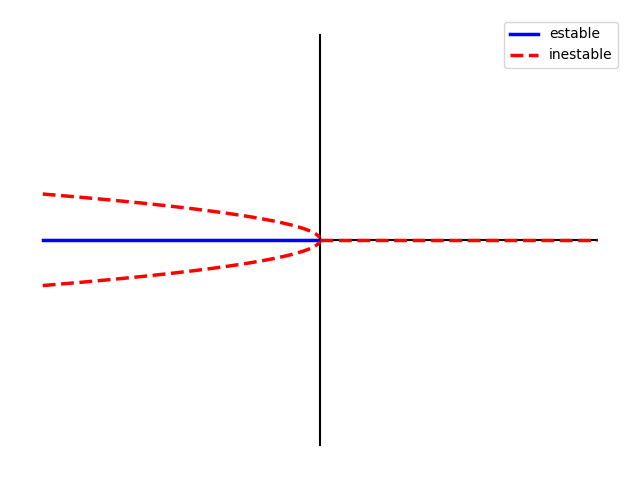
\includegraphics[scale=0.5]{img/9.png}
    \end{figure}
\end{solution}

\begin{exercise}
    Ídem para
    \begin{enumerate}
        \item $x' = \mu x - 4x^3$.
        \item $x' = x+\frac{\mu x}{1+x^2}$.
    \end{enumerate}
\end{exercise}

\begin{solution}
    Solo se va a resolver el apartado (b). Sea $f(\mu,x) = x+\frac{\mu x}{1+x^2}$. Se tiene que
    \begin{align*}
        f(\mu,x) = 0 \iff x = 0 \textup{ ó } \mu = -1-x^2.
    \end{align*}
    Por tanto, el conjunto de los equilibrios del sistema es
    \[\{(\mu,0) \in\R^2 \colon \mu \in \R\} \cup \{(-1-x^2,x) \in\R^2 \colon x \in \R\}.\]
    Además, \[\frac{\partial f}{\partial x}(\mu,x) = 1+\frac{\mu(1+x^2)-2\mu x^2}{(1+x^2)^2} = 1+\frac{\mu(1 -x^2)}{(1+x^2)^2}.\] Se tiene que $\frac{\partial f}{\partial x}(\mu,0) = 1+\mu$ para todo $\mu\in\R$, mientras que \[\frac{\partial f}{\partial x}(-1-x^2,x) = 1-\frac{(1+x^2)(1-x^2)}{(1+x^2)^2} = 1-\frac{1-x^2}{1+x^2} = \frac{1+x^2-1+x^2}{1+x^2} = \frac{2x^2}{1+x^2}\] para todo $x\in\R$. Por tanto, el conjunto de los equilibrios asintóticamente estables e hiperbólicos es
    \[\{(\mu,0) \in\R^2 \colon \mu < -1\},\]
    mientras que el conjunto de los equilibrios inestables, repulsores e hiperbólicos es
    \[\{(\mu,0) \in\R^2 \colon \mu > -1\} \cup \{(-1-x^2,x) \in\R^2 \colon x \neq 0\}.\]
    El equilibrio $(-1,0)$ no es hiperbólico. Observando la gráfica de $f(-1,x) = x-\frac{x}{1+x^2}$ se deduce que $(-1,0)$ es semiestable por la derecha.
    \begin{figure}[H]
        \centering
        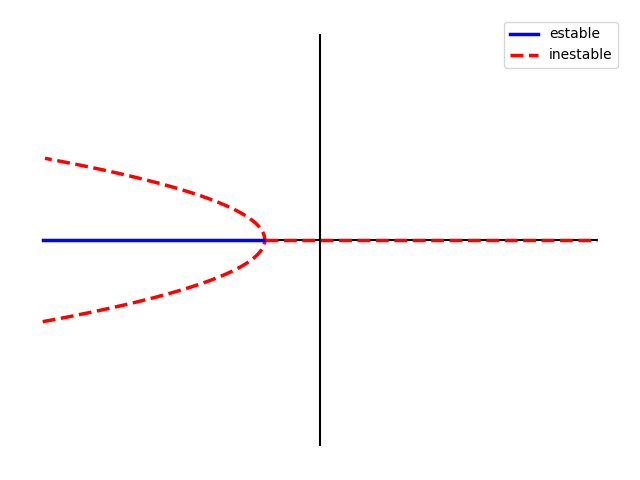
\includegraphics[scale=0.5]{img/10.png}
    \end{figure}
\end{solution}

\begin{exercise}
    Ídem para
    \begin{enumerate}
        \item $x' = \mu - 3x^2$.
        \item $x' = \mu x - \frac{x}{1+x}$.
    \end{enumerate}
\end{exercise}

\begin{solution}
    Solo se va a resolver el apartado (a). Sea $f(\mu,x) = \mu-3x^2$. Se tiene que
    \begin{align*}
        f(\mu,x) = 0 \iff \mu = 3x^2.
    \end{align*}
    Por tanto, el conjunto de los equilibrios del sistema es
    \[\{(3x^2,x) \in\R^2 \colon x \in \R\}.\]
    Además, $\frac{\partial f}{\partial x}(\mu,x) = -6x$. Se tiene que $\frac{\partial f}{\partial x}(3x^2,x) = -6x$ para todo $x \in \R$, así que el conjunto de los equilibrios asintóticamente estables e hiperbólicos es
    \[\{(3x^2,x) \in\R^2 \colon x > 0\},\]
    mientras que el conjunto de los equilibrios inestables, repulsores e hiperbólicos es
    \[\{(3x^2,x) \in\R^2 \colon x < 0\}.\] 
    El equilibrio $(0,0)$ no es hiperbólico. Observando la gráfica de $f(0,x) = -3x^2$ se deduce que $(0,0)$ es semiestable por la derecha.
    \begin{figure}[H]
        \centering
        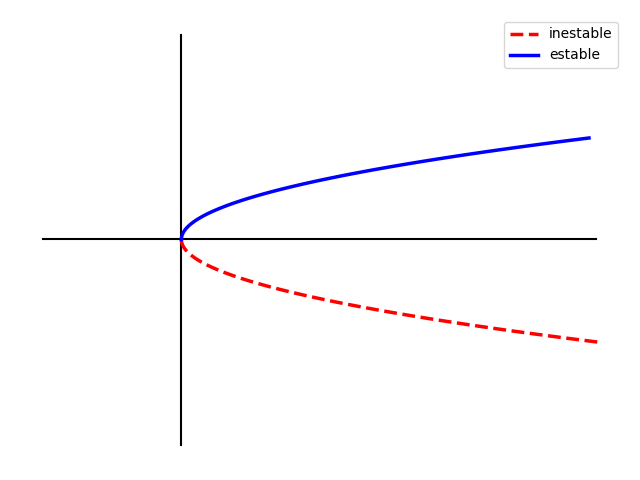
\includegraphics[scale=0.5]{img/11.png}
    \end{figure}
\end{solution}

\begin{exercise}
    Ídem para
    \begin{enumerate}
        \item $x' = 5-\mu e^{-x^2}$.
        \item $x' = \mu x -\frac{x}{1+x^2}$.
    \end{enumerate}
\end{exercise}

\begin{solution}
    Solo se va a resolver el apartado (b). Sea $f(\mu,x) = \mu x-\frac{x}{1+x^2}$. Se tiene que
    \begin{align*}
        f(\mu,x) = 0 \iff x = 0 \textup{ ó } \mu = \frac{1}{1+x^2}.
    \end{align*}
    Por tanto, el conjunto de los equilibrios del sistema es
    \[\{(\mu,0) \in\R^2 \colon \mu \in \R\} \cup \bigl\{\bigl(\frac{1}{1+x^2},x\bigr) \colon x \in \R\bigr\}.\]
    Además, \[\frac{\partial f}{\partial x}(\mu,x) = \mu - \frac{1+x^2-2x^2}{(1+x^2)^2} = \mu + \frac{x^2-1}{(1+x^2)^2}.\] Se tiene que $\frac{\partial f}{\partial x}(\mu, 0) = \mu-1$ para todo $\mu \in \R $, mientras que
    \[\frac{\partial f}{\partial x}\bigl(\frac{1}{1+x^2},x\bigr) = \frac{1+x^2+x^2-1}{(1+x^2)^2} = \frac{2x^2}{(1+x^2)^2}\]
    para todo $x \in \R$. En consecuencia, el conjunto de los equilibrios asintóticamente estables e hiperbólicos es
    \[\{(\mu,0) \in\R^2 \colon \mu < 1\},\]
    mientras que el conjunto de los equilibrios inestables, repulsores e hiperbólicos es
    \[\{(\mu,0) \in\R^2 \colon \mu > 1\} \cup \bigl\{\bigl(\frac{1}{1+x^2},x\bigr) \colon x \neq 0\bigr\}.\]
    El equilibrio $(1,0)$ no es hiperbólico. Observando la gráfica de $f(1,x) = x-\frac{x}{1+x^2}$ se deduce que $(1,0)$ es semiestable por la izquierda.
    \begin{figure}[H]
        \centering
        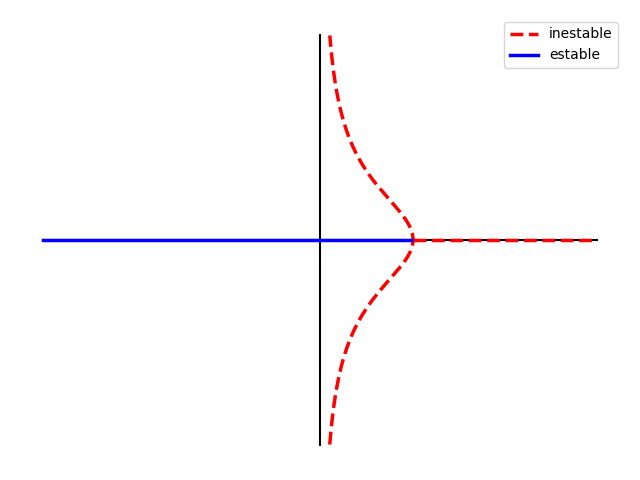
\includegraphics[scale=0.5]{img/12.png}
    \end{figure}
\end{solution}

\begin{exercise}
    Ídem para
    \begin{enumerate}
        \item $x' = x+\tgh(\mu x)$.
        \item $x' = \mu x + \frac{x^3}{1+x^2}$.
    \end{enumerate}
\end{exercise}

\begin{solution}
    Solo se va a resolver el apartado (a). Sea $f(\mu,x) = x+\tgh(\mu x)$. Si $x \neq 0$, se tiene que
    \begin{align*}
        f(\mu,x) = 0 &\iff x + \frac{e^{\mu x} - e^{-\mu x}}{e^{\mu x} + e^{-\mu x}} = 0 \iff  \frac{e^{2\mu x} - 1}{e^{2\mu x} + 1}= -x \iff e^{2\mu x} - 1 = -x(e^{2\mu x} + 1) \\
        &\iff e^{2\mu x}(1+x) = 1-x \iff 2\mu x = \log(1-x)-\log(1+x) \\
        &\iff \mu = \frac{ \log(1-x)-\log(1+x)}{2x}.
    \end{align*}
    Todo lo anterior es válido si $x \in (-1,0) \cup (0,1)$. También se tiene que $f(\mu,0) = 0$. Por tanto, el conjunto de los equilibrios del sistema es
    \[\bigl\{\bigl(\frac{ \log(1-x)-\log(1+x)}{2x},x\bigr)\in\R^2\colon x \in (-1,0)\cup (0,1)\bigr\} \cup \{(\mu,0) \in\R^2\colon \mu \in \R\}.\]
    Además, \begin{align*}
        \frac{\partial f}{\partial x}(\mu,x) &= 1+\frac{2\mu e^{2\mu x}(e^{2\mu x} +1) -2\mu e^{2\mu x} (e^{2\mu x}-1)}{(e^{2\mu x}+1)^2} = 1+\frac{4\mu e^{2\mu x}}{(e^{2\mu x}+1)^2}.
    \end{align*}
    Por tanto, $\frac{\partial f}{\partial x}(\mu,0) = 1+\frac{4\mu}{4} = 1+\mu$. Sea $x \in (-1,0)\cup(0,1)$ y sea $\mu = \frac{ \log(1-x)-\log(1+x)}{2x}$. Entonces $2\mu x = \log(\frac{1-x}{1+x})$ y $4\mu = \frac{2}{x}\log(\frac{1-x}{1+x})$, luego 
    \begin{align*}
        \frac{\partial f}{\partial x}\bigl(\frac{ \log(1-x)-\log(1+x)}{2x},x\bigr) &= 1+\frac{\frac{2}{x}\frac{1-x}{1+x}\log(\frac{1-x}{1+x})}{(\frac{1-x}{1+x}+1)^2}.
    \end{align*}
    Representando la gráfica de la función anterior se observa que $\frac{\partial f}{\partial x}(\frac{ \log(1-x)-\log(1+x)}{2x},x) > 0$ para todo $x \in (-1,0)\cup (0,1)$. En consecuencia, el conjunto de los equilibrios asintóticamente estables e hiperbólicos es
    \[\{(\mu,0)\in \R^2 \colon \mu < -1\},\]
    mientras que el conjunto de los equilibrios inestables, repulsores e hiperbólicos es
    \[\bigl\{\bigl(\frac{ \log(1-x)-\log(1+x)}{2x},x\bigr)\in\R^2\colon x \in (-1,0)\cup (0,1)\bigr\} \cup \{(\mu,0)\in \R^2 \colon \mu > -1\}.\]
    El equilibrio $(-1,0)$ no es hiperbólico. Observando la gráfica de $f(-1,x) = x+\tgh(-x)$ se deduce que $(-1,0)$ es semiestable por la derecha.
    \begin{figure}[H]
        \centering
        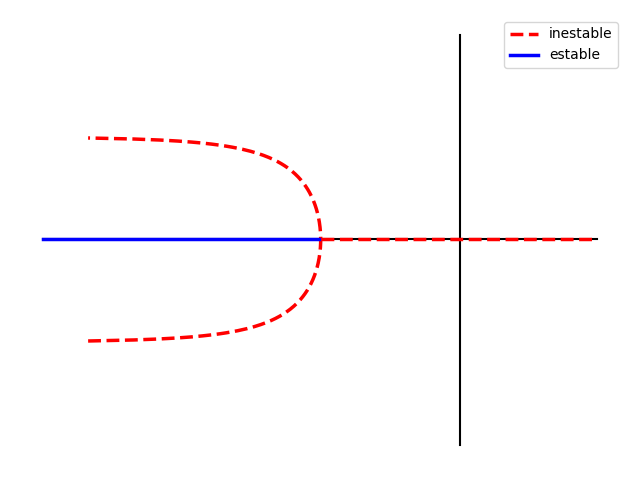
\includegraphics[scale=0.5]{img/13.png}
    \end{figure}
\end{solution}

\begin{exercise}
    Una partícula viaja por la semirrecta $x \geq 0$ con velocidad $x' = -x^c$, siendo $c$ una constante real.
    \begin{enumerate}
        \item Encontrar todos los valores de $c$ que hacen que el origen $x = 0$ sea un punto crítico estable.
        \item Sea $c$ tal que $x = 0$ es estable. ¿Puede alcanzar una partícula el origen en tiempo finito? Concretamente, ¿cuánto tarda una partícula en viajar desde $x = 1$ hasta $x = 0$ (como función de $c$)?
    \end{enumerate}
\end{exercise}

\begin{solution}
    Sea $f(x) = -x^c$, $x \geq 0$.
    \begin{enumerate}
        \item En primer lugar, $x = 0$ es un punto crítico del sistema si y solo si $c > 0$. En ese caso, como $f(x) < 0$ para todo $x > 0$, se tiene que $x = 0$ es asintóticamente estable.
        \item Sea $c > 0$, de manera que $x = 0$ es estable. Para cada $x_0 > 0$, considérese el problema
        \[
            (P) \ \begin{cases}
                x'=-x^c, \qquad t \geq 0, \\
                x(0) = x_0.
            \end{cases}
        \]
        Si $c = 1$, la única solución del problema anterior es $x(t)= x_0e^{-t}$, que satisface $x(t) > 0$ para todo $t \geq 0$. Por tanto, la partícula no alcanza el origen en tiempo finito en este caso.
        
        Supóngase ahora que que $c \neq 1$. Las soluciones de la ecuación $x'=-x^c$ son de la forma
        \[x(t) = \bigl((K-t)(1-c)\bigr)^{\frac{1}{1-c}}, \qquad t \geq 0,\]
        con $K \in\R$ constante. Se tiene que
        \[x(0) = x_0 \iff K^{\frac{1}{1-c}}(1-c)^{\frac{1}{1-c}} = x_0 \iff K = \frac{x_0^{1-c}}{1-c},\]
        con lo que queda determinada la única solución del problema $(P)$. Se observa que la partícula alcanza el origen en el tiempo $t = K$, que solo tiene sentido si $K \geq 0$, es decir, si $0 < c < 1$. En ese caso, el tiempo que tarda la partícula en viajar desde $x = x_0 = 1$ hasta $x = 0$ es $t = \frac{1}{1-c}$.
    \end{enumerate}
\end{solution}

\begin{exercise}
    Demostrar que una ecuación diferencial ordinaria autónoma $x'=f(x)$ no puede tener soluciones periódicas. Para ello, suponer que $x$ es una solución periódica no trivial y que $T>0$ es su periodo. Llegar a una contradicción considerando $\int_t^{t+T}f(x(s))x'(s)\, ds$.
\end{exercise}

\begin{solution}
    Por reducción al absurdo, sea $x$ una solución $T$-periódica no trivial (es decir, no constante) de la ecuación $x'=f(x)$. Sea $F$ una primitiva de $f$. Entonces
    \[(F \circ x)'(s) = F'(x(s))x'(s) = f(x(s))x'(s)\]
    para todo $s \in \R$, luego
    \[\int_t^{t+T}f(x(s))x'(s)\, ds = \int_t^{t+T}(F\circ x)'(s) = F(x(t+T))-F(x(t)) = F(x(t))-F(x(t))=0\]
    para todo $t \in \R$, donde en la penúltima igualdad se usa que $x$ es $T$-periódica. Ahora bien, como $x'= f(x)$, entonces
    \[\int_t^{t+T}f(x(s))x'(s)\, ds = \int_t^{t+T}x'(s)^2\, ds.\]
    Se tiene que $x'(s)^2 \geq 0$ para todo $s \in [t,t+T]$ y su integral en dicho intervalo es nula, luego $x'(s) = 0$ para todo $s \in [t,t+T]$. En consecuencia, $x$ es constante en $[t,t+T]$, y como $x$ es $T$-periódica, entonces también es constante en $\R$, que es una contradicción.
\end{solution}

\begin{exercise}
    Se considera un depósito cilíndrico con sección de área constante $A$. El agua entra en el depósito con una velocidad constante $k$ y lo abandona por un pequeño orificio de área $a$ en el fondo del depósito. De acuerdo con la ley de Torricelli, el agua escapa a través del agujero con una velocidad que es, en cada instante, igual a $\alpha a \sqrt{2gh(t)}$, siendo $h(t)$ la altura que alcanza el agua que hay en el depósito en dicho instante; $g$ es la aceleración de la gravedad y $\alpha$, un coeficiente que satisface $0'5\leq \alpha \leq 1$.
    \begin{enumerate}
        \item Probar que la altura del agua en el depósito, $h(t)$, satisface la ecuación diferencial
        \[\frac{dh}{dt} = \frac{k-\alpha a \sqrt{2gh}}{A}.\]
        \item Determinar la altura de equilibrio del agua, $h_e$, y probar que es estable (nótese que $h_e$) no depende de $A$.
    \end{enumerate}
\end{exercise}

\begin{solution}
    \hfill
    \begin{enumerate}
        \item La velocidad a la que varía la altura del agua en el depósito será algo así como
        \[\frac{dh}{dt} = \frac{\textup{velocidad a la que entra el agua} - \textup{velocidad a la que sale el agua}}{\textup{área de las secciones del depósito}} = \frac{k-\alpha a \sqrt{2gh}}{A}.\]
        \item Lo de siempre: se considera la función $f(h) = \frac{k-\alpha a\sqrt{2gh}}{A}$ y se hallan sus ceros y su derivada. Por un lado,
        \[f(h) = 0 \iff \frac{k-\alpha a \sqrt{2gh}}{A} = 0 \iff \sqrt{2gh} = \frac{k}{\alpha a} \iff h = \frac{k^2}{2g\alpha^2 a^2}.\]
        Por otro lado,
        \[f'(h) = -\frac{\frac{2g\alpha a}{A}}{2\sqrt{2gh}} = -\frac{g\alpha a}{A\sqrt{2gh}}.\]
        Sea $h_e = \frac{k^2}{2g\alpha^2 a^2}$. Como
        \[f'(h_e) = -\frac{g\alpha a}{A\frac{k}{\alpha a}} = -\frac{g\alpha^2a^2}{Ak}<0,\]
        entonces el equilibrio del agua es asintóticamente estable.
    \end{enumerate}
\end{solution}

\addtocounter{exercise}{1}

\begin{exercise}
    La población de una especie de peces, medida en miles de individuos, se rige por la ecuación diferencial autónoma
    \[\frac{dx}{dt} = g(x),\]
    donde la función $g$ viene dada por la expresión
    \[g(x) = -x(x-1)(x-2)(x-3),\]
    cuya gráfica se representa en la siguente figura:
    \begin{figure}[H]
        \centering
        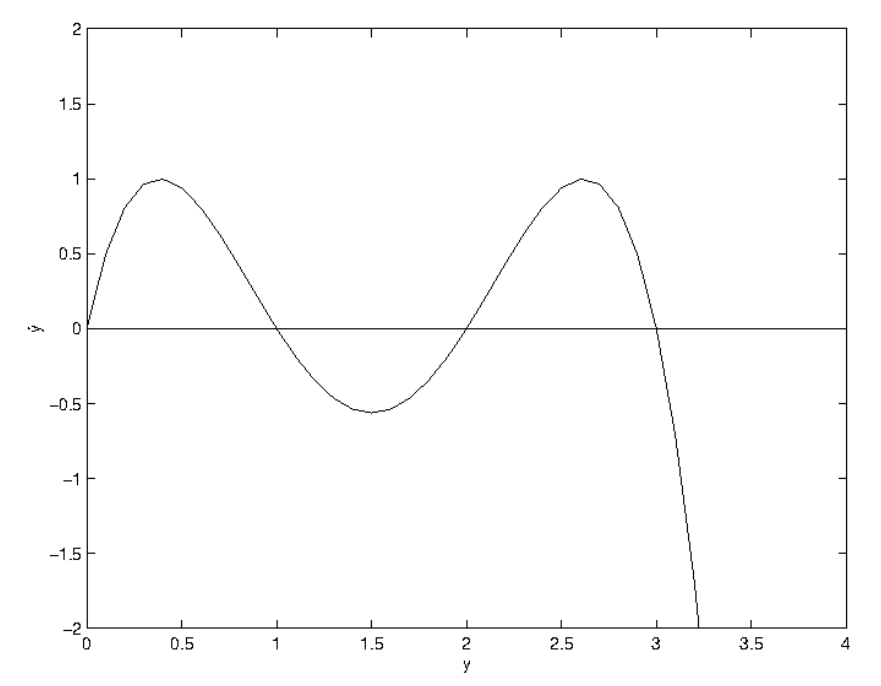
\includegraphics[scale = 0.4]{img/14.png}
    \end{figure}
    \begin{enumerate}
        \item Estudiar las soluciones de equilibrio y su estabilidad.
        \item Describir la dinámica general de la población, es decir, cómo evolucionará dependiendo de la condición inicial.
        \item Supóngase que se somete la población a explotación pesquera, con una tasa de capturas proporcional al número de individuos. Se denomina $\alpha$ al cociente de proporcionalidad. ¿Qué valores de $\alpha$ serían admisibles para no extinguir con seguridad la especie?
        \item Dibujar de forma aproximada el diagrama de bifurcación correspondiente al apartado anterior. A la vista del diagrama, ¿qué valores de $\alpha$ serían aconsejables?
    \end{enumerate}
\end{exercise}

\begin{solution}
    \hfill
    \begin{enumerate}
        \item Las soluciones de equilibrio son, claramente, $l_1 = 0$, $l_2 = 1$, $l_3 = 2$ y $l_4 = 3$. En la gráfica de $g$ se observa que $l_1$ es inestable y repulsor, $l_2$ es asintóticamente estable, $l_3$ es inestable y repulsor, y $l_4$ es asintóticamente estable.
        \item Sea $x_0 \geq 0$ la condición inicial. En virtud de lo afirmado en el apartado anterior, se tiene que:
        \begin{itemize}
            \item Si $x_0 = 0$, la población es siempre nula.
            \item Si $0 < x_0 < 1$, la población tenderá a estabilizarse en $1000$ peces.
            \item Si $x_0 = 1$, la población es siempre de $1000$ peces.
            \item Si $1 < x_0 < 2$, la población tenderá a estabilizarse en $1000$ peces.
            \item Si $x_0 = 2$, la población es siempre de $2000$ peces.
            \item Si $2 < x_0 < 3$, la población tenderá a estabilizarse en $3000$ peces.
            \item Si $x_0 = 3$, la población es siempre de $3000$.
            \item Si $x_0 > 3$, la población tenderá a estabilizarse en $3000$ peces.
        \end{itemize}
        \item En las nuevas circunstancias de explotación pesquera, la población se peces se rige por la ecuación diferencial autónoma
        \[\frac{dx}{dt} = g(x) - \alpha x.\]
        Para hallar los equilibrios del nuevo modelo, se estudian los puntos de corte de la gráfica de $g$ con las rectas $y = \alpha x$, con $\alpha > 0$.
        \begin{figure}[H]
            \centering
            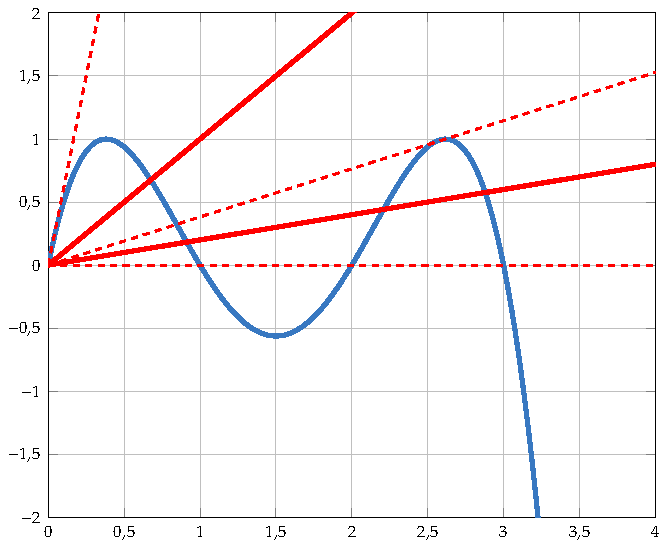
\includegraphics[scale = 0.7]{plot3/main.pdf}
        \end{figure}
        Se tiene que $g'(0) = 6$ y que el segundo máximo de $g$ es alcanzado en $x = \frac{3}{2}+\frac{\sqrt{5}}{2}$. De esto y la gráfica de arriba se obtienen las siguientes conclusiones:
        \begin{itemize}
            \item Si $\alpha \geq 6$, entonces la recta $y = \alpha x$ solo corta a la gráfica de $g$ en $x = 0$. En ese caso, como la gráfica queda por debajo de la recta, $0$ es un equilibrio asintóticamente estable, así que la población de peces se extingue.
            \item Si $\frac{2}{3+\sqrt{5}} <  \alpha < 6$, entonces hay dos equilibrios. El primero es $x = 0$, inestable y repulsor porque la gráfica queda por encima de la recta en un entorno a la derecha $0$. El segundo equilibrio es asintóticamente estable, pues la gráfica queda por encima de la recta en un entorno a la izquierda del equilibrio, y queda por debajo de la recta en un entorno a la derecha del equilibrio.
            \item Si $\alpha = \frac{2}{3+\sqrt{5}}$, entonces hay tres equilibrios. El primero ($x = 0$) es inestable y repulsor, el segundo es asintóticamente estable, y el tercero ($x = \frac{3}{2}+\frac{\sqrt{5}}{2}$) es semiestable por la derecha.
            \item Si $0<\alpha < \frac{2}{3+\sqrt{5}}$, entonces hay cuatro equilibrios. Los mismos razonamientos de índole geométrica prueban que el primero ($x=0$) es inestable y repulsor, el segundo es asintóticamente estable, el tercero es inestable y repulsor, y el cuarto es asintóticamente estable.
        \end{itemize}
        Se concluye que si $0 < \alpha < 6$, entonces la población de peces no se extingue.
        \item A la vista del diagrama de bifurcación, los valores aconsejables de $\alpha$ son aquellos con $\frac{2}{3+\sqrt{5}} < \alpha <6$.
        \begin{figure}[H]
            \centering
            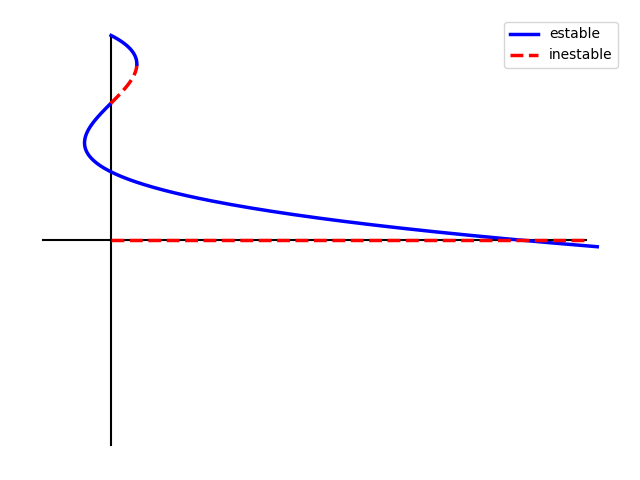
\includegraphics[scale = 0.5]{img/15.png}
        \end{figure}
    \end{enumerate}
\end{solution}

\end{document}